\documentclass[deposito, acronym, symbols]{fei}

%\usepackage{glossaries}
\usepackage{subcaption} 
\usepackage{float}
%\usepackage{units}
\usepackage[portuguese]{algorithm2e}
\usepackage{biblatex}
\usepackage{amsmath}
\usepackage{listings}
\lstset{frame=tb,
language=Matlab,
aboveskip=3mm,
belowskip=3mm,
showstringspaces=false,
columns=flexible,
basicstyle={\small\ttfamily},
numbers=left,
numberstyle=\tiny\color{gray},
keywordstyle=\color{blue},
commentstyle=\color{dkgreen},
stringstyle=\color{mauve},
breaklines=true,
breakatwhitespace=true,
tabsize=4,
frame=shadowbox,
literate={á}{{\'a}}1 {ã}{{\~a}}1 {é}{{\'e}}1 {ê}{\^e}1 {ç}{\c{c}}1 {í}{\i}1 {ú}{\'u}1 {ó}{{\'o}}1 {õ}{{\~o}}1 {Á}{{\'A}}1 {É}{{\'E}}1, }
%%
\usepackage{color}
\definecolor{dkgreen}{rgb}{0,0.6,0}
\definecolor{mauve}{rgb}{0.58,0,0.82}
\usepackage[utf8]{inputenc}
\usepackage{chngcntr} %Faz com que o numero das notas de rodape aumente crescentemente.
\usepackage{appendix}
\counterwithout{footnote}{chapter}% "
\usepackage{siunitx}
\sisetup{output-exponent-marker=\ensuremath{\mathrm{e}}} %Escrita que precede cada entrada na lista de ilustrações.
\renewcommand{\cftfigurepresnum}{Figura }
\setlength{\cftfigurenumwidth}{5.7em}

\usepackage{titling}

%\makeglossaries
%%\newacronym[] {achpt} {ACT} {Aparecido ChupeTão}

\newacronym[longplural=Associações Brasileiras de Normas Técnicas]{abnt}{ABNT}{Associação Brasileira de Normas Técnicas}

\newacronym{ibge}{IBGE}{Instituto Brasileiro de Geografia e Estatística}

\newacronym{ashrae}{ASHRAE}{\textit{American Society of Heating, Refrigerating and Air-Conditioning Engineers}}

\newacronym{nbr}{NBR}{Norma Brasileira}

\newacronym{pmv}{PMV}{\textit{Predicted Mean Vote}}
	
\newacronym{ppd}{PPD}{\textit{Predicted Percentage of Dissatisfied}}
		
\newacronym{vgd}{VGD}{Ventilação Geral Diluidor}
		
\newacronym{vgl}{VGL}{Ventilação Local Exaustora}
		
\newacronym{cfd}{CFD}{\textit{Computational Fluid Dynamics}}
		
\newacronym{pcb}{PCB}{\textit{Printed Circuit Board}}
		
\newacronym{sms}{SMS}{\textit{Short Message Service}}
		
%\newglossaryentry{pi}{parent=greek,type=symbols,name={\ensuremath{\pi}},sort=p,description={número irracional que representa [razão entre a circunferência de qualquer círculo e seu diâmetro]}}
		


\title{Estudo de um amortecedor de automóvel utilizando elemento de mola 2D e arranjo de dados}
\author{ Felipe Estevão Coquito de Mello \\ Gabriel Mola da Silva \\ Netuno Trindade Torrente Rovaroto \\ Vitoria Fedatto Stefaneli}
\cidade{São Bernardo do Campo}
\instituicao{Centro Universitário FEI}

\addbibresource{Referencias.bib}
%\bibliographystyle{plain}
\bibliography{Referencias}
\graphicspath{ {Imagens/}, {Tabelas/}}

\begin{document}
\maketitle

\listoffigures
\listoftables

\chapter{Introdução e Objetivos}

Com o avanço tecnológico e a complexidade de resolver os desafios do mundo real, tornou-se necessário abordagens mais eficientes e completas para solucionar tais problemas. Portanto, é fundamental o aprendizado de ferramentas computacionais para uma melhor análise e observação dos casos.

 Neste trabalho será avaliado o comportamento de um sistema que simula o amortecimento de um automóvel utilizando o software de análise numérica MATLAB. O cálculo do deslocamento das molas e das forças aguentadas de um amortecedor de um carro é comum na indústria e para isso, com o auxílio do MATLAB, faremos análises pertinentes para a estrutura que escolhemos.

\chapter{Fundamentação Téorica}

Nesta seção serão detalhados os conceitos básicos para entendimento geral do projeto desenvolvido, tais como: conceito de amortecimento e para criação dos códigos.

\section{Amortecedores hidráulicos}

Amortecedores são formados por dois componentes que juntos controlam e diminuem as variações do solo. O amortecedor hidráulico ou convencional trabalha com um pistão dentro de um tubo que contêm óleo, envolto por uma mola.

Tal componente é de suma importância para a segurança do veículo e de seus passageiros, pois está ligado diretamente à frenagem e estabilidade do veículo, principalmente em curvas. Portanto é fundamental que as peças estejam em perfeito estado para garantir a segurança de todos.

As molas do amortecedor de um carro absorvem a energia do impacto que posteriormente será controlada pelo amortecedor, suavizando assim os movimentos de retornos das molas às suas posições originais.

\begin{figure}[!htb]
 \centering
    \caption{Amortecedor Hidraulico.}
    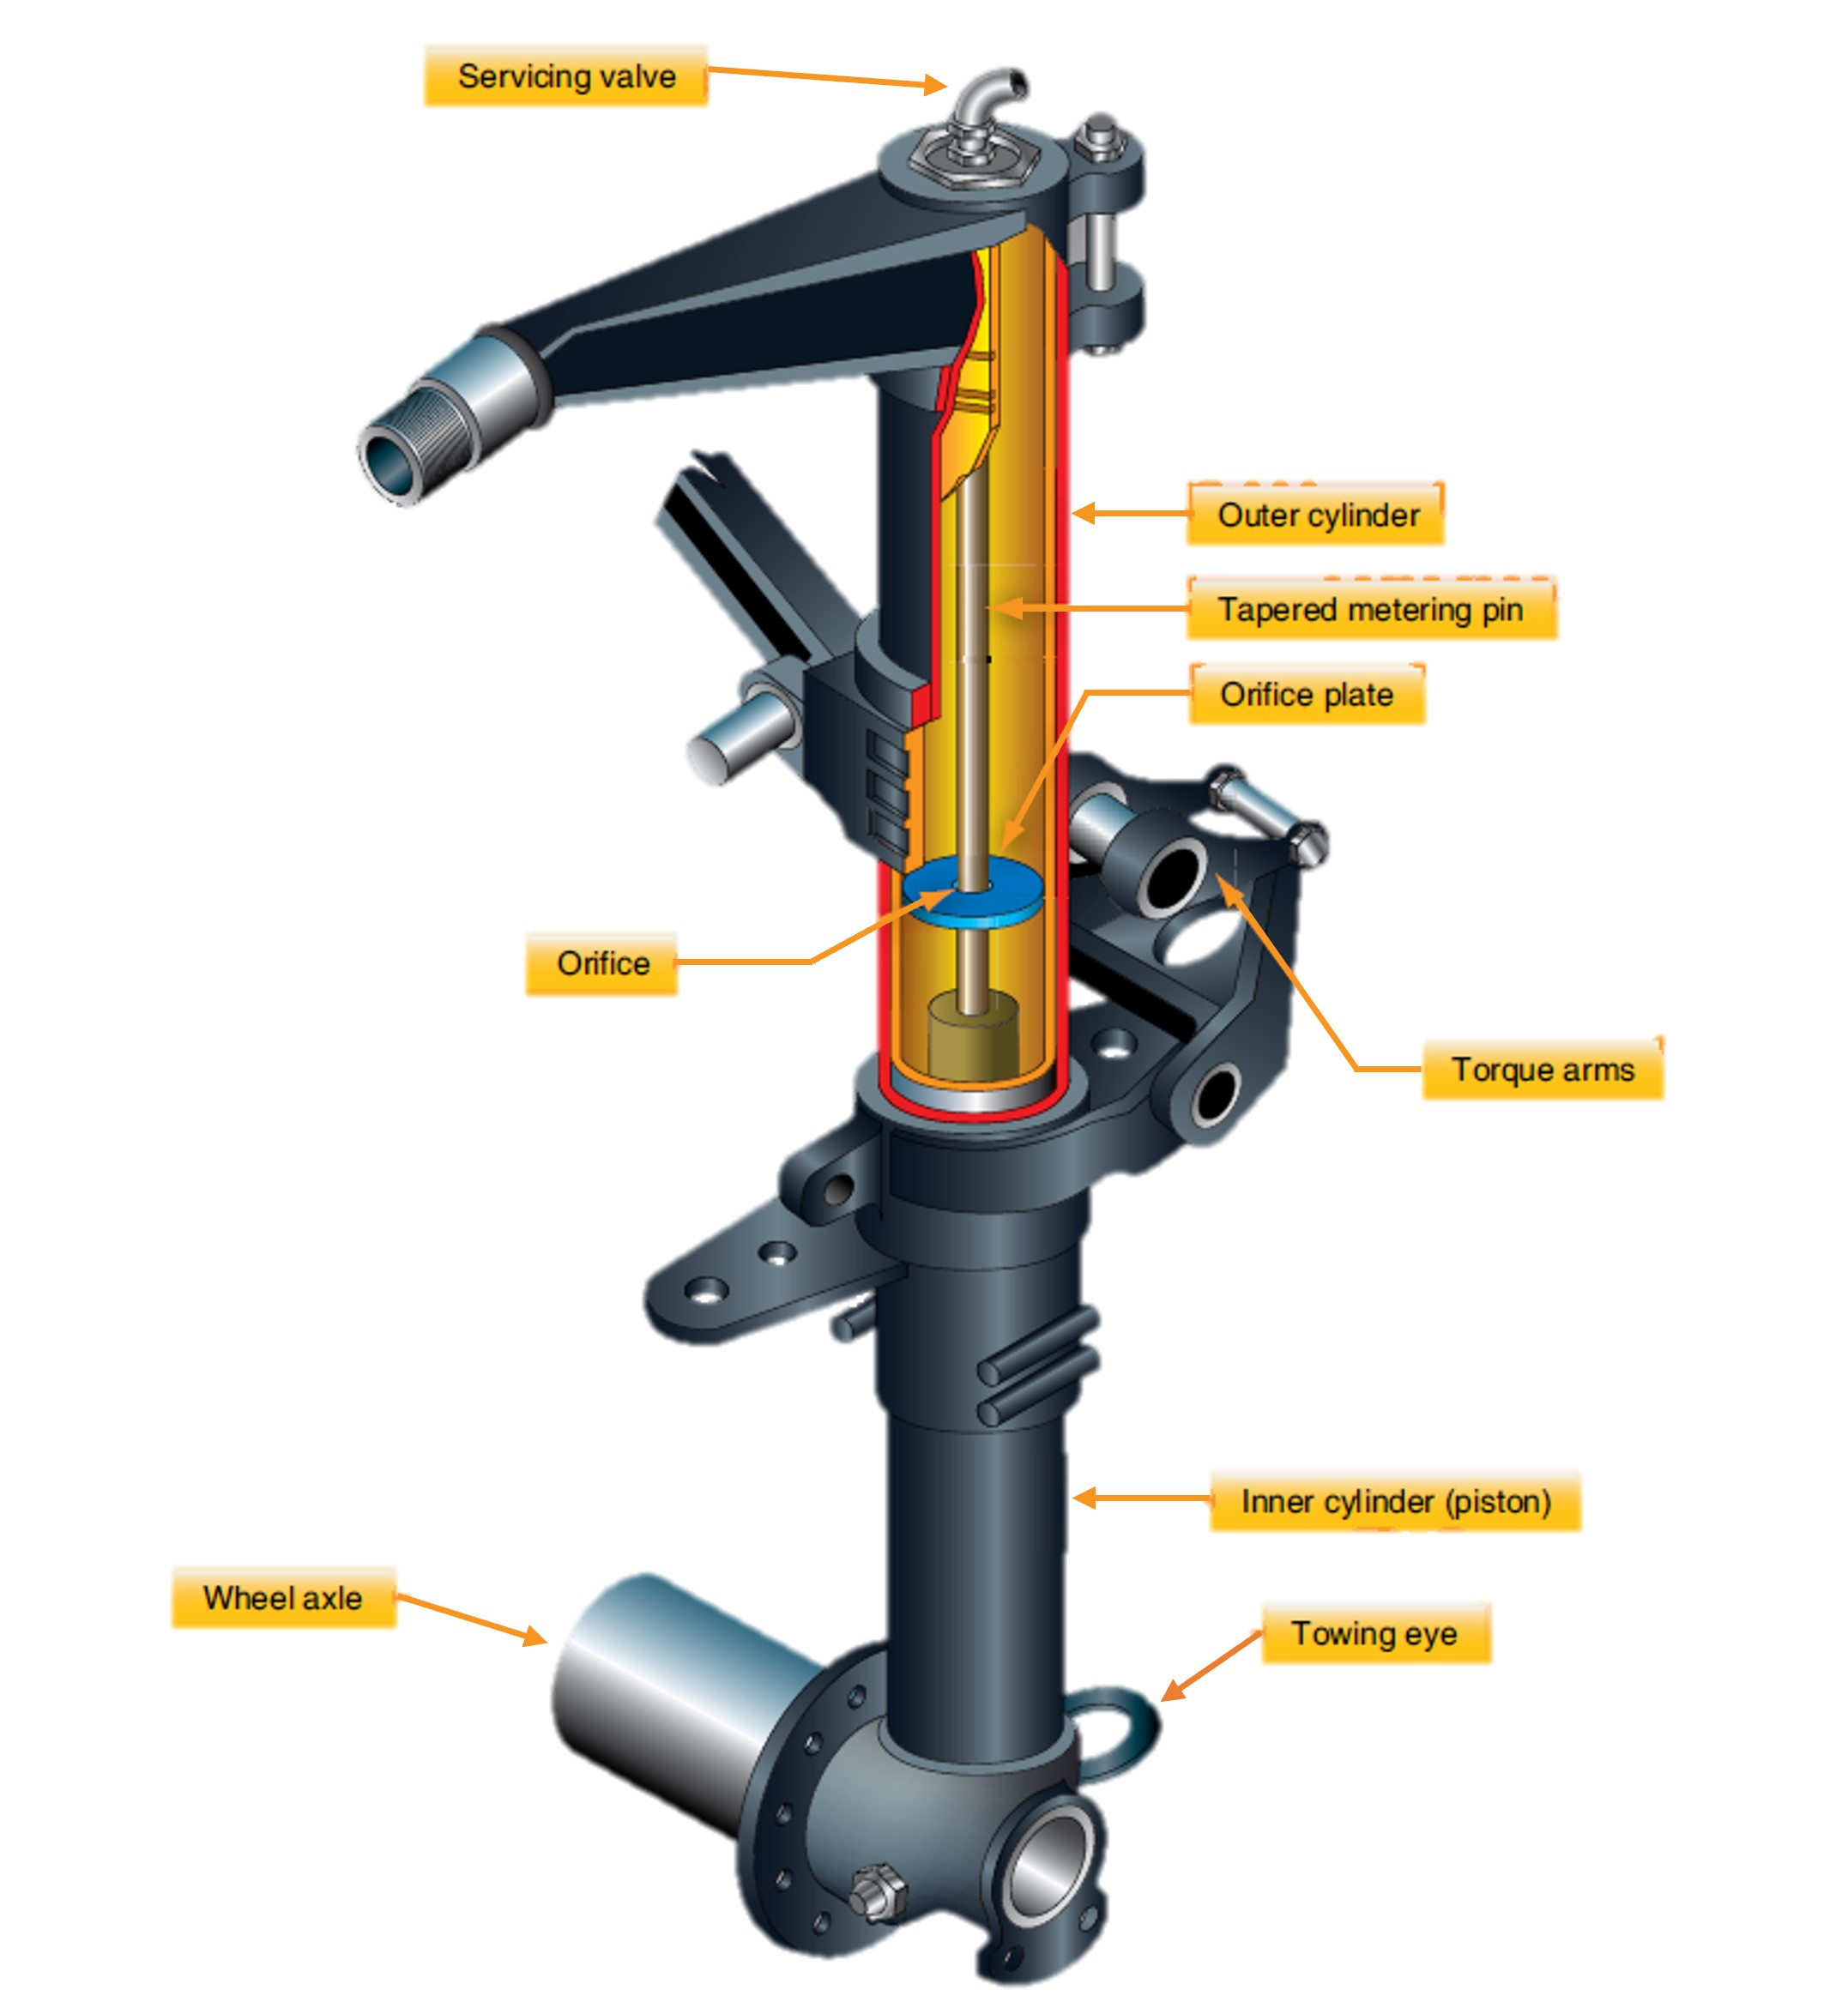
\includegraphics[width=0.7\linewidth]{Imagens/hidraulico.jpg}
    \smallcaption{Fonte: Hangarmma}
    \label{fig:hidraulica}
 \end{figure}

\section{Elemento de mola 2D}
O Método dos Elementos Finitos consiste em utilizar métodos numéricos aplicados em uma geometria com carregamentos e restrições e dividi-la em pequenas partes que passam a representar o sistema todo do problema. O método supõe que a partir de um número infinito de variáveis desconhecidas sejam substituídas por um certo número de elementos com comportamento conhecido e definido. 

Para que seja possível fazer a equação de equilíbrio de um sistema é necessário o uso do Teorema do Mínimo do Funcional PI que é um sistema que envolve as variações de funções. O teorema mostra que, para um sistema com n graus de liberdade, existem infinitos estados, e cada estado é representado por um PI. Ele mostra, também, que a posição de equilíbrio é representada num ponto crítico, ou seja, quando as derivadas parciais de PI forem iguais a zero. 

Para o uso de elementos de mola se faz certas hipóteses simplificadoras, sendo elas: as molas estão em regime linear, adotar pequenas deformações e apenas presença de tração e compressão e a presença de apenas 2 graus de liberdade por nó. A representação de molas para os sistemas mecânicos elásticos utiliza métodos como o método da sobreposição ou montagem. Esse método consiste na formação de uma unidade fundamental que nada mais é que uma matriz que se repete várias vezes e representa como cada mola influencia no conjunto todo. Também é chamada de matriz de rigidez do elemento. 

A matriz de rigidez do elemento é obtida ao analisar o comportamento de um único elemento da estrutura, isolando-o. A matriz de rigidez da estrutura, entretanto, é obtida através da soma (sobreposição) das diversas matrizes de elementos. Para a montagem desta matriz por sobreposição é necessário dar “endereços”, escolhidos aleatoriamente, aos elementos para se posicionarem na matriz da estrutura.

O problema analisado nesta atividade é um elemento de mola 2D, sendo assim existem outras matrizes importantes para a análise do comportamento da estrutura, como a matriz de transformação de coordenadas. Esta matriz, como o nome diz, transforma as coordenadas locais em globais, para que seja possível montar a matriz K de rigidez dos elementos. Uma vez obtida, a energia potencial elástica armazenada pode ser calculada em qualquer coordenada, pois não depende do sistema de coordenadas. 

Além desta matriz, para fazer a análise computacional de uma mola 2D, é preciso determinar matrizes de identidade, incidência, localização e propriedades.

\chapter{Projeto}

Neste trecho será apresentado a estrutura escolhida pelo grupo e o código completo para realização da sua análise.

\section{Desenho Esquematizado}

O modelo prático consiste em uma associação de 10 elementos de Rigidez, conforme indicado nas figuras abaixo, sendo dois deles com rigidez extremamente alta (barras 7 e 8), e os outros 8 elementos com rigidez variando de 0,5 kN/m até 2 kN/m. O sistema apresenta um apoio fixo no nó 1 e um apoio móvel no nó 4. 

Utilizamos o Software Autocad para desenvolver e implementar o projeto descrito na Figura [\ref{fig: Estrutura}], assim como utilizamos o software MATLAB para analisarmos o deslocamento do sistema com duas forças atuantes (7kN e 3 kN) a um ângulo de 45°. 

\begin{figure}[!htb]
 \centering
    \caption{Estrutura Base.}
    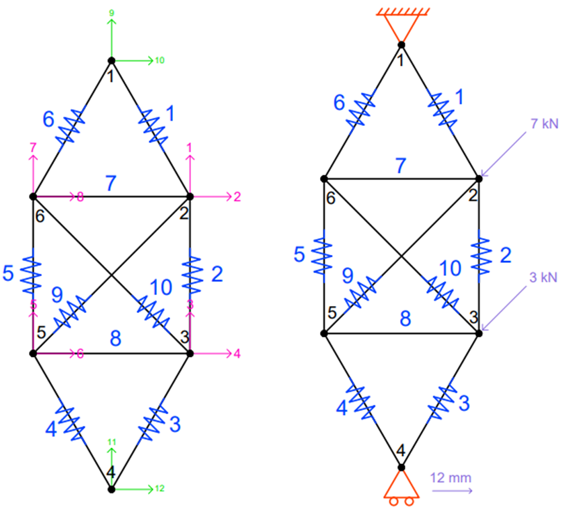
\includegraphics[width=0.6\linewidth]{Imagens/Estrutura 1.png}
    \smallcaption{Fonte: Autor}
    \label{fig: Estrutura}
 \end{figure}

\section{Códigos}

Os códigos foram desenvolvidos pelo professor Mohammad Shaterzadeh, utilizando o software MATLAB que utiliza a linguagem Fortran. O código utilizado para a simulação está descrito abaixo:

\subsection{Código Principal}

\begin{lstlisting}
clearvars; clc; close all;

%==============================
% ENTRADA DE DADOS DA ESTRUTURA
%==============================
nEL = 10;        % Quantidade total de elementos
nNO = 6;        % Quantidade total de nós
nGL = 2;        % Quantidade GL por nó

alpha = 1:8;    % GLs desconhecidos
beta  = 9:12;   % GLs conhecidos (fixos ou prescritos)

% Matriz de Identidade (ID)
ID(1,1:nNO) = [10 2 4 12 6 8]; % Graus de liberdade em X
ID(2,1:nNO) = [9 1 3 11 5 7];  % Graus de liberdade em Y

% Matriz de Incidência (IN)
IN(1,1:nEL) = [1 2 3 4 5 6 6 5 5 3];
IN(2,1:nEL) = [2 3 4 5 6 1 2 3 2 6];

% Matriz de Localização (LM)
LM(1,1:nEL) = [10 2 4 12 6 10 8 6 2 8];
LM(2,1:nEL) = [9 1 3 11 5 9 7 5 1 7];
LM(3,1:nEL) = [2 4 12 6 8 8 2 4 6 4];
LM(4,1:nEL) = [1 3 11 5 7 7 1 3 5 3];

% Matriz de Propriedades (PROP)
PROP(1,1:nEL) = [2 0.5 1 1 0.5 2 1000 1000 1.5 1.5];
PROP(2,1:nEL) = [-60 -90 -120 -120 -90 -60 0 0 -45 -135];

% Vetor de carregamentos externos
F = zeros(nNO*nGL,1);
F(alpha) = [-5 -5 -2.1 -2.1 0 0 0 0];

% Vetor de graus de liberdade (GLs)
X = zeros(nNO*nGL,1);
X(beta) = [0 0 0 12];

% Geometria original
COORD(1,1:nNO) = [1 2 2 1 0 0];
COORD(2, ...
    1:nNO) = [3 2 1 0 1 2];
escala = 0.04;

%==============================
% CÁLCULO DO MEF
%==============================
% Calcula as matriz de rigidez global para cada elemento
for el = 1:nEL
  Ke(:,:,el) = CalculaMatrizRigidezElemento(el,PROP);
end

% Monta a matriz de rigidez GLOBAL
Kg = zeros(nNO*nGL);
for el = 1:nEL
  Kg(LM(:,el),LM(:,el))=Kg(LM(:,el),LM(:,el))+Ke(:,:,el);
end

% Verifica se a solução existe e é única
det(Kg(alpha,alpha));   % É diferente de zero -> OK!  

% Solução dos GLs desconhecidos
X(alpha) = Kg(alpha,alpha)\(F(alpha)-Kg(alpha,beta)*X(beta));

% Cálculo das reações de apoio
F(beta) = Kg(beta,alpha)*X(alpha) + Kg(beta,beta)*X(beta);

% Verificação das condições de equilíbrio
Fx = F(1:2:end);
sum(Fx);  
Fy = F(2:2:end);
sum(Fy);

% Cálculo da energia potencial
for el = 1 : nEL
  Xel = X(LM(:,el));
  U(el) = .5*Xel'*Ke(:,:,el)*Xel;
end

% Cálculo das forças nos elementos
for el = 1 : nEL
  Ke_local = PROP(1,el)*[ 1 0 -1 0; 0 0 0 0;...
                         -1 0  1 0; 0 0 0 0];
  T = CalculaMatrizTransformacao(el,PROP);
  Xel = X(LM(:,el));
  Xel_local = T * Xel;
  Felem(:,el) = Ke_local * Xel_local;
end

%==============================
% PLOTAGEM
%==============================
figure(1); hold on;
% Plota os nós
for i = 1 : nNO
  plot(COORD(1,i), COORD(2,i), 'bo');
end
box on; grid on; axis equal;
% Plota os elementos
for el = 1 : nEL
  plot(COORD(1,IN(:,el)),COORD(2,IN(:,el)),'b--','DisplayName','Original');
end

% Geometria deformada
DEF(1,:) = COORD(1,:) + escala*X(ID(1,:))';
DEF(2,:) = COORD(2,:) + escala*X(ID(2,:))';

% Plota os nós deslocados
for i = 1 : nNO
  plot(DEF(1,i), DEF(2,i), 'ro');
end
box on; grid on; axis equal;
% Plota os elementos deformados
for el = 1 : nEL
  plot(DEF(1,IN(:,el)),DEF(2,IN(:,el)),'r','linewidth',3,'DisplayName','Deformada');
end

title('GEOMETRIA ORIGINAL E DEFORMADA','Fontsize',20);

\end{lstlisting}


\subsection{Cálculo da Matriz de Rigidez dos Elemento}

\begin{lstlisting}
function Ke = CalculaMatrizRigidezElemento(el,PROP)

m = cosd(PROP(2,el));
n = sind(PROP(2,el));

Ke = PROP(1,el)*[ m^2  m*n -m^2 -m*n;
                  m*n  n^2 -m*n -n^2;
                 -m^2 -m*n  m^2  m*n;
                 -m*n -n^2  m*n  n^2];
\end{lstlisting}


\subsection{Cálculo da Matriz de Transformação}

\begin{lstlisting}
function T = CalculaMatrizTransformacao(el,PROP)

% Matriz Transformação
m = cosd(PROP(2,el));
n = sind(PROP(2,el));

T = [ m n  0 0;
     -n m  0 0;
      0 0  m n;
      0 0 -n m];
      
\end{lstlisting}

\chapter{Montagem das Matrizes}

\section{Matriz de Identidade (ID)}

\begin{table}[!hb]
 \centering
    \caption{Matriz de Identidade (ID).}
    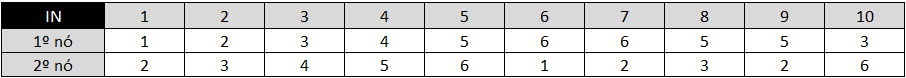
\includegraphics[width=1\linewidth]{Tabelas/Matriz de Incidencia.png}
    \smallcaption{Fonte: Autor}
    \label{tab: Matriz ID}
 \end{table}

Para preencher a Matriz de Identidade (ID), que está indicada na Tabela [\ref{tab: Matriz ID}], foi necessário definir quais são os graus de liberdade verticais e horizontais, assim como indicado na Figura [\ref{fig: Estrutura ID}].

\begin{figure}[!htb]
 \centering
    \caption{Estrutura e seus Graus de Liberdade.}
    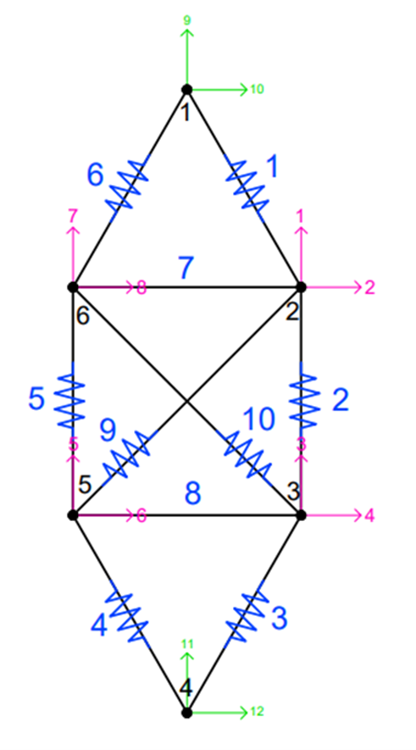
\includegraphics[width=0.5\linewidth]{Imagens/Estrutura ID.png}
    \smallcaption{Fonte: Autor}
    \label{fig: Estrutura ID}
 \end{figure}

\section{Matriz de Localização (LM)}

\begin{table}[!htb]
 \centering
    \caption{Matriz de Localização (LM).}
    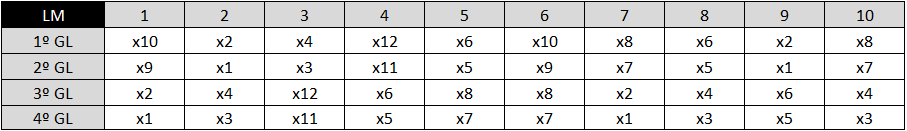
\includegraphics[width=1\linewidth]{Tabelas/Matriz de Localizacao.png}
    \smallcaption{Fonte: Autor}
    \label{tab: Matriz LM}
 \end{table}

Para preencher a Matriz de Localização (LM), que está indicada na Tabela [\ref{tab: Matriz LM}], foi necessário definir quais são os graus de liberdade verticais e horizontais de um primeiro nó, e os mesmos parâmetros de um segundo nó, representando assim o elemento que entre estes dois pontos escolhidos, assim como indicado na Figura [\ref{fig: Estrutura LM}].

\begin{figure}[!htb]
 \centering
    \caption{Estrutura e seus Graus de Liberdade Totais.}
    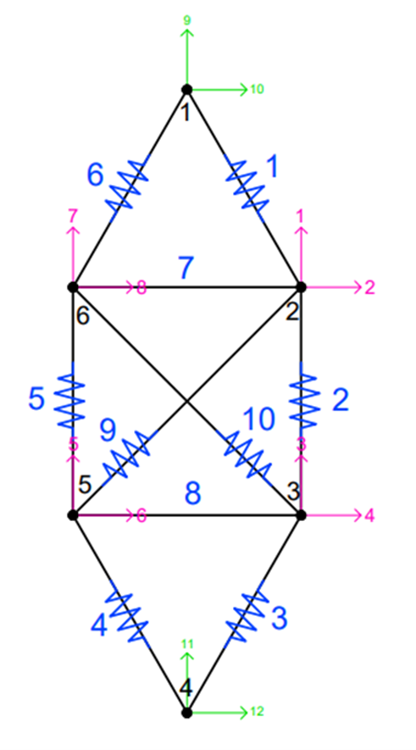
\includegraphics[width=0.5\linewidth]{Imagens/Estrutura ID.png}
    \smallcaption{Fonte: Autor}
    \label{fig: Estrutura LM}
 \end{figure}

\section{Matriz de Incidência (IN)}

\begin{table}[!htb]
 \centering
    \caption{Matriz de Incidência (IN).}
    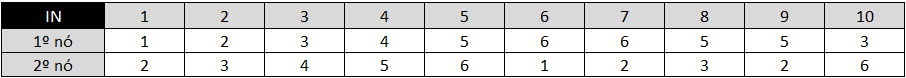
\includegraphics[width=1\linewidth]{Tabelas/Matriz de Incidencia.png}
    \smallcaption{Fonte: Autor}
    \label{tab: Matriz IN}
 \end{table}
 
Preenchemos a Matriz de Incidência (IN), que está indicada na Tabela [\ref{tab: Matriz IN}], representando um elemento de rigidez. Através da posição de um nó inicial, até um nó final, é possível indicar a posição deste elemento, assim como indicado na Figura [\ref{fig: Estrutura IN}].

\begin{figure}[!htb]
 \centering
    \caption{Elementos e Nós.}
    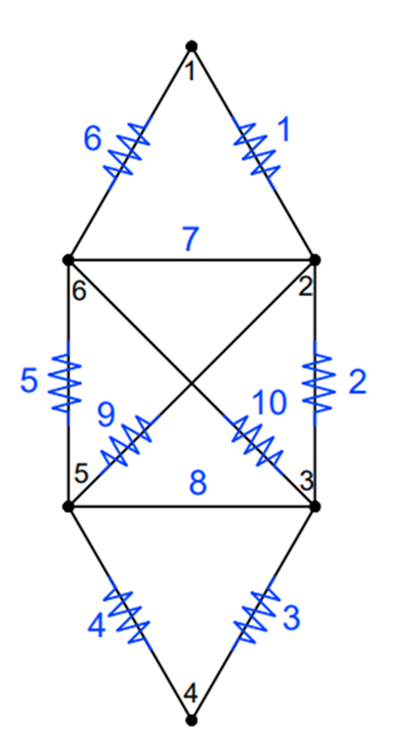
\includegraphics[width=0.5\linewidth]{Imagens/Estrutura IN.png}
    \smallcaption{Fonte: Autor}
    \label{fig: Estrutura IN}
 \end{figure}
 
\section{Matriz de Proppreidades (PROP)}

\begin{table}[!htb]
 \centering
    \caption{Matriz de Proppreidades (PROP).}
    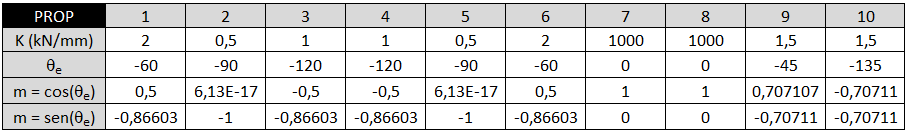
\includegraphics[width=1\linewidth]{Tabelas/Matriz de Propriedades.png}
    \smallcaption{Fonte: Autor}
    \label{tab: Matriz PROP}
 \end{table}

Para preencher a Matriz de Propriedades (PROP), que está indicada na Tabela [\ref{tab: Matriz PROP}], foi necessário definir o ângulo entre uma referência horizontal X, até um elemento de rigidez, adotando sempre o sentido anti-horário, assim como indicado na Figura [\ref{fig: Estrutura PROP}].

\begin{figure}[!htb]
 \centering
    \caption{Angulo dos Elementos.}
    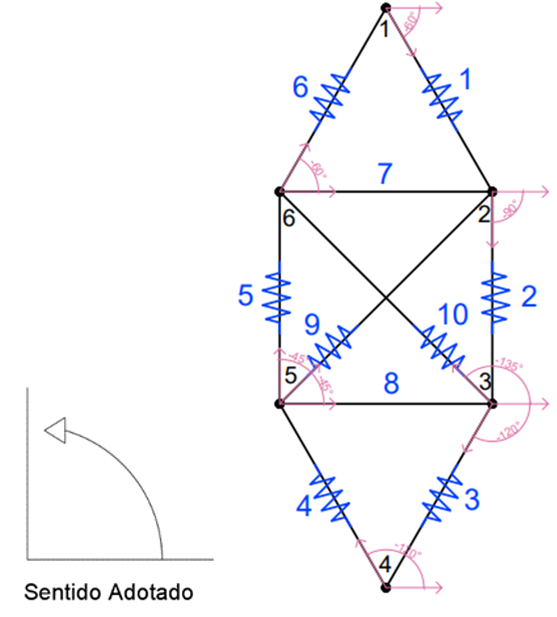
\includegraphics[width=0.8\linewidth]{Imagens/Estrutura PROP.png}
    \smallcaption{Fonte: Autor}
    \label{fig: Estrutura PROP}
 \end{figure}
 
\section{Matriz de Coordenadas (COORD)}

\begin{table}[!htb]
 \centering
    \caption{Matriz de Coordenadas (COORD).}
    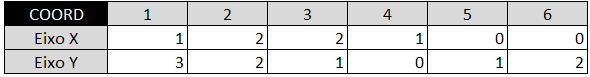
\includegraphics[width=1\linewidth]{Tabelas/Matriz de Cordenada.png}
    \smallcaption{Fonte: Autor}
    \label{tab: Matriz COORD}
 \end{table}

Para preencher a Matriz de Coordenas (COORD), que está indicada na Tabela [\ref{tab: Matriz COORD}], foi necessário traçar linhas verticais e horizontais que cruzassem os nós, e selecionar os números das linhas que ao serem cruzadas representassem a posição destes nós em relação a um referencial X e Y adotado, assim como indicado na Figura [\ref{fig: Estrutura COORD}].

\begin{figure}[!htb]
 \centering
    \caption{Coordenadas dos Nós.}
    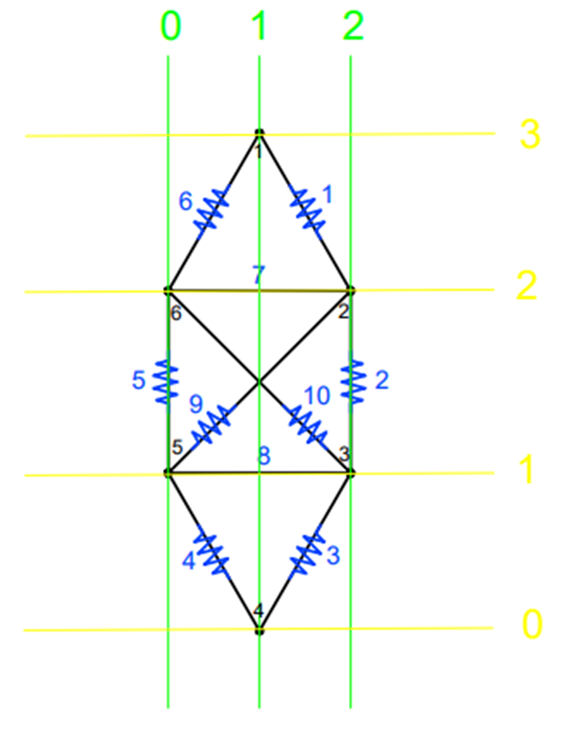
\includegraphics[width=0.7\linewidth]{Imagens/Estrutura CORD.png}
    \smallcaption{Fonte: Autor}
    \label{fig: Estrutura COORD}
 \end{figure}

\chapter{Resultado e Discussão}

Nesse trecho será feita uma breve análise sobre as matrizes de saídas do código, no caso, as matrizes de força, deformação e energia potencial. Além disso, faremos apontamentos sobre o resultado final do experimento, comentando a respeito do gráfico da geometria deformada.
 
\section{Forças aplicadas}

\begin{table}[!htb]
 \centering
    \caption{Matriz de Forças nos Nós.}
    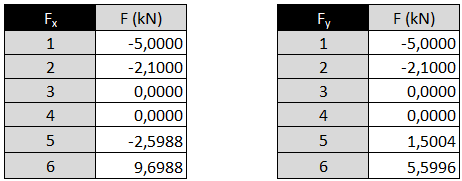
\includegraphics[width=0.7\linewidth]{Tabelas/Foracas Aplicadas.png}
    \smallcaption{Fonte: Autor}
    \label{tab: Forças aplicadas}
 \end{table}

Primeiramente obtivemos através do MATLAB a Matriz de Forças [\ref{tab: Forças aplicadas}] no eixo X e Y em cada nó de nossa estrutura, foi possível observar que os nós com maior concentração de forças foram o primeiro e o sexto.

\section{Forças nos elementos}

\begin{table}[!htb]
 \centering
    \caption{Matriz de Forças nos Elementos.}
    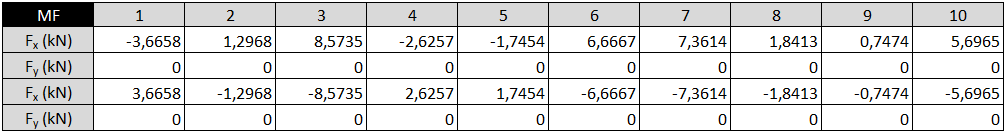
\includegraphics[width=1\linewidth]{Tabelas/Matriz Calculo das Forcas nos Elementos.png}
    \smallcaption{Fonte: Autor}
    \label{tab: Forças nos elementos}
 \end{table}

Obtivemos também a Matriz de Forças em Cada Elemento do Sistema [\ref{tab: Forças nos elementos}], sendo estas referentes as coordenadas locais, nos permitindo apontar que os elementos que tem maior força concentrada são os elementos 3, 7 e 6. Nenhum elemento apresenta Forças no eixo Y pois seria caracterizado como Flambagem, algo que o sistema não apresenta.

\newpage
\section{Deformações}

\begin{figure}[!h]
 \centering
    \caption{Gráfico da Deformação.}
    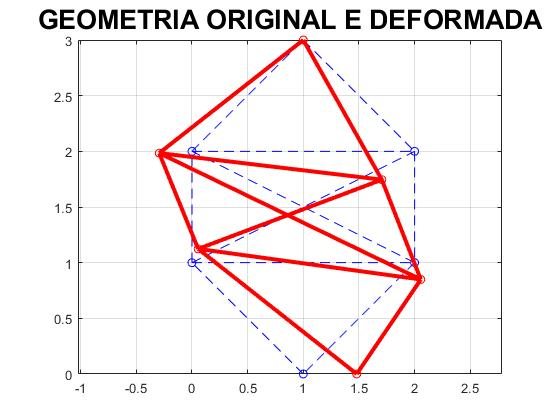
\includegraphics[width=0.6\linewidth]{Imagens/Deform.jpg}
    \smallcaption{Fonte: Autor}
    \label{fig: Deformação}
 \end{figure}

A partir do Gráfico [\ref{fig: Deformação}] retirado do MATLAB, foi possível observar como seria a deformação de nossa estrutura com as forças definidas, isso é de grande ajuda para ter uma melhor visualização do projeto, nos permitindo ter uma ideia geral de como seriam esses deslocamentos, tendo maior facilidade do que na análise por tabelas.
 
\begin{table}[!htb]
 \centering
    \caption{Matriz de Deformações.}
    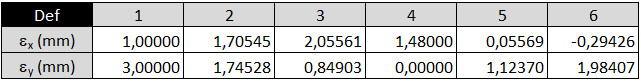
\includegraphics[width=0.8\linewidth]{Tabelas/Deformacao.png}
    \smallcaption{Fonte: Autor}
    \label{tab: Deformormação}
 \end{table}

Foi retirada do MATLAB as Matrizes das Deformações em cada nó da Estrutura [\ref{tab: Deformormação}], que ao observarmos podemos analisar que os pontos que sofreram a maior deformação no eixo X foram o terceiro e o quarto nó, já no eixo 4 foram o primeiro e sexto nó. 

\section{Energia Potencial}

\begin{table}[!htb]
 \centering
    \caption{Matriz Cálculo da Energia Potencial.}
    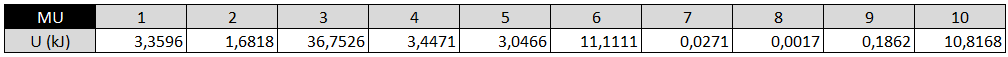
\includegraphics[width=1\linewidth]{Tabelas/Matriz Calculo da Energia Potencial.png}
    \smallcaption{Fonte: Autor}
    \label{tab: Energia Potencial}
 \end{table}

Ao logo de nosso experimento também calculamos a Energia Potencial em cada elemento de nossa estrutura [\ref{tab: Energia Potencial}], possibilitando analisarmos a distribuição e concentração de energia potencial, os elementos que apresentaram maior energia potencial foram 3, 6 e 10.
 
\chapter{Conclusão}

Como dito acima o trabalho foi realizado para estudar o comportamento das molas de um amortecedor de um automóvel em movimento. E concluiu-se que ao admitirmos um deslocamento inicial de 12 mm na base do amortecedor, por exemplo, o carro passando por um buraco em uma rua, e juntamente com as forças horizontais e verticais aplicados pelo próprio carro, as deformações das molas são consideráveis. Portanto, os resultados encontrados são fidedignos aos resultados esperados para esse componente. 

\printbibliography[type=online]
\nocite{*}

\end{document}